% \documentclass[8pt, handout]{beamer}
\documentclass[8pt]{beamer}
\usetheme{metropolis}
\usepackage{minted}
\usepackage{mathtools}
\usepackage{graphicx}

\setminted{fontsize=\small,baselinestretch=1}

\newfontfamily\mfont[Ligatures=TeX]{Fira Sans UltraLight}
\newcommand{\muted}[1]{{\mfont#1}}
\newcommand{\remark}[1]{{\footnotesize#1}}
\newcommand{\Reals}{\mathbb{R}}
\newcommand{\rand}{\,\wedge\,}
\newcommand{\ror}{\,\vee\,}
\newcommand{\dom}{\operatorname{Dom}}
\def\fs{\vskip0ex}

\title[Haskell na produkcji]{Haskell na produkcji}
\subtitle{czyli czy warto sięgać po niestandardowe narzędzia}

\author{Tomasz Tylec} % Your name
\institute[IFR/M-ZF]
{
IF Research Polska (Gdańsk) / Mazars-Zettafox (Paris)
\medskip\hspace{1ex}$\vert$\hspace{1ex}
\textit{tomasz.tylec@ifresearch.pl}
}
\date{11 listopada 2018} % Date, can be changed to a custom date

\begin{document}

\begin{frame}
\titlepage % Print the title page as the first slide
\end{frame}

\begin{frame}
\frametitle{Outline}
\tableofcontents
\end{frame}

\section{Reguły klasyfikujące}

\def\ruleform{
Rozważać będziemy reguły postaci:
\[
  c_1 \rand c_2 \rand \dots \rand c_n,
\]
gdzie $c_i$ jest postaci $X \in \{\dots\}$,
lub $X\in (a, b)$.}

\begin{frame}[fragile]
  \frametitle{Reguły}

  \begin{block}{Definicja}
    \fs
    \emph{Regułą} nazywamy predykat, wyrażenie logiczne, które
    każdemu elementowi w zbiorze danych przypisuje wartość \emph{prawda}
    lub \emph{fałsz}.
  \end{block}

  \begin{block}{Przykład}
    \fs
    Dane:

    \begin{tabular}{r | r r r}
      index & A & B & C \\
      \hline
      0 & low & high & low \\
      \alert<3->{1} & \alert<3->{low} & \alert<3->{low} & \alert<3->{low} \\
      2 & high & low & high \\
      \alert<3->{3} & \alert<3->{medium} & \alert<3->{low} & \alert<3->{high}
    \end{tabular}

    \pause

    Reguła: $A \in \{\text{low}, \text{medium}\} \rand B \in \{\text{low}\}$
  \end{block}

  \ruleform

\end{frame}

\begin{frame}
  \frametitle{Algebra reguł}
  \begin{block}{Reguły tworzą zbiór częściowo uporządkowany}
    \fs
    $r \le q$ jeśli dla każdego wiersza dla którego $q$ jest prawdziwe, $r$
    też jest prawdziwe.

    Przykłady:
    \begin{itemize}
      \item
        $
        A \in \{\text{low}\} \rand B \in \{\text{low}\} \le
        A \in \{\text{low}, \text{medium}\} \rand B \in \{\text{low}\}
        $
      \item ale $A\in \{\text{low}\}$ oraz $B \in \{high\}$ jest są w relacji
        porządku.
    \end{itemize}
  \end{block}

  \pause

  \begin{block}{Reguły można ze sobą łączyć}
    \fs
    Jeśli $r, q$ są regułą to $r \rand q$ też jest regułą. Wtedy
    $r\rand q \le r$ oraz $r\rand q \le q$.

    {\footnotesize \ruleform\par}

    Jeśli $r, q$ są regułą to $r \ror q$ definiujemy jako najmniejszą
    (w sensie $\le$) regułę spełniającą: $r \le r\ror q$ oraz $q \le r\ror q$.
  \end{block}
\end{frame}

\begin{frame}[standout]
  \frametitle{Zadanie}

  Mając do dyspozycji zbiór sklasyfikowanych danych, znaleźć niewielki zbiór \emph{najlepszych}
  reguł, względem pewnej funkcji oceniającej (\emph{score function}).
\end{frame}

\begin{frame}
  \frametitle{Metoda I: przeszukiwanie drzewa}
  Zaczynając od zbioru najogólniejszych nietrywialnych reguł $a_1, a_2, \dots,
  a_k$, tworzymy reguły postaci:
  \begin{itemize}
  \item $a_2 \rand a_5$,
  \item $a_5 \rand a_{10} \rand a_{143}$,
  \item $a_{242} \rand a_{743} \rand a_{342} \rand a_{1233}$,
  \item itd.
  \end{itemize}
  wybierając tylko te najlepsze.

  \pause
  \bigskip
  {\footnotesize
  \begin{columns}[T]
    \begin{column}{.4\linewidth}
        \begin{tabular}{r | r r r}
          index & A & B & C \\
          \hline
          \alert<3>{0} & \alert<3>{low} & \alert<3>{hig } & \alert<3>{low} \\
          \alert<3,4,5>{1} & \alert<3,4,5>{low} & \alert<3,4,5>{low} & \alert<3,4,5>{low} \\
          \alert<4>{3} & \alert<4>{high} & \alert<4>{low} & \alert<4>{high} \\
          \alert<3,4,5>{4} & \alert<3,4,5>{medium} & \alert<3,4,5>{low} & \alert<3,4,5>{high}
        \end{tabular}
    \end{column}
    \begin{column}{.6\linewidth}
        \begin{align*}
          \dom(A) &= \{\text{low, medium, high}\} \\
          \dom(B) &= \{\text{low, high}\} \\
          \dom(C) &= \{\text{low, medium, high}\}
        \end{align*}
    \end{column}
  \end{columns}
  \par}
  $\alert<3>{a_1 = A\in\{\text{low, medium}\}},
   \alert<4>{a_3 = B\in\{\text{low}\}}$
  $\alert<5>{r = a_1\rand a_3 = A\in\{\text{low, medium}\} \rand B\in\{\text{low}\}}$
\end{frame}


\begin{frame}
  \frametitle{Metoda II:  przeszukiwanie podzbiorów}

  Każdy element zbioru danych $x_i$ odpowiada regule $r(x_i)$-- takiej, która wybiera
  dokładnie ten element. Tworzymy reguły postaci:

  \begin{itemize}
  \item $r(x_{10}) \ror r(x_{31})$,
  \item $r(x_1) \ror r(x_{45}) \ror r(x_{321}) \ror r(x_{1421}) \ror r(x_{2352}) \ror
    r(x_{31002})$
  \item itp.
  \end{itemize}
  wybierając najlepsze.

  \pause
  \bigskip
  {\footnotesize
  \begin{columns}[T]
    \begin{column}{.4\linewidth}
        \begin{tabular}{r | r r r}
          index & A & B & C \\
          \hline
          {0} & {low} & {high} & {low} \\
          \alert<3,5>{1} & \alert<3,5>{low} & \alert<3,5>{low} & \alert<3,5>{low} \\
          \alert<5>{3} & \alert<5>{low} & \alert<5>{low} & \alert<5>{high} \\
          \alert<4,5>{4} & \alert<4,5>{medium} & \alert<4,5>{low} & \alert<4,5>{high}
        \end{tabular}
    \end{column}
    \begin{column}{.6\linewidth}
        \begin{align*}
          \dom(A) &= \{\text{low, medium, high}\} \\
          \dom(B) &= \{\text{low, high}\} \\
          \dom(C) &= \{\text{low, medium, high}\}
        \end{align*}
    \end{column}
  \end{columns}
  \par}
  $\alert<3>{a_1 = A\in\{\text{low}\} \rand B\in\{\text{low}\} \rand C\in\{\text{low}\}}$
  $\alert<4>{a_2 = A\in\{\text{medium}\} \rand B\in\{\text{low}\} \rand C\in\{\text{high}\}},$
  $\alert<5>{r = a_1\rand a_2 = A\in\{\text{low, medium}\} \rand
    B\in\{\text{low}\}\rand C\in\{\text{low, high}\}}$
\end{frame}

\begin{frame}
  \frametitle{Problemy}
  Obie metody wymagają:
  \begin{itemize}
  \item szybkiego liczenia funkcji \emph{score} (wiele reguł do sprawdzenia);
  \item efektywnej implementacji algebry reguł (wiele reguł do skonstruowania);
  \item stosowania heurystycznych optymalizacji.
  \end{itemize}

  \pause

  W konsekwencji:
  \begin{itemize}
    \item kod będzie się często zmieniał na etapie tworzenia prototypu
    \item nie wiadomo z góry, która reprezentacja reguł będzie optymalna
    \item może istnieć więcej niż jeden sposób heurystycznej optymalizacji
      przeszukania
    \item może nie istnieć globalnie najefektywniejsze rozwiązanie
  \end{itemize}

  Z drugiej strony, opis algorytmu jest bardzo prosty.
\end{frame}

\section{Implementacja w Haskellu}

\subsection{Dlaczego Haskell?}

\begin{frame}[fragile]
  \frametitle{Czym jest Haskell?}
  General-purpose, purely functional programming language with non-strict
  semantics and strong static typing [wikipedia]
  \pause
  \begin{itemize}
  \item \emph{strongly typed:} wszystko ma określony typ;
    kompilator statycznie sprawdza zgodność typów;
    brak domyślnych konwersji między typami.
    \medskip
\begin{minted}{haskell}
pi  :: Double
sin :: Double -> Double
\end{minted}
      {\footnotesize
      podobnie jak w matematyce:
      $\pi \in \mathbb{R}, sin\colon \mathbb{R} \to \mathbb {R}$}

  \pause
  \item \emph{pure:} brak zmiennych i efektów ubocznych
    \medskip
\begin{minted}{haskell}
a = 5
a = 3         -- to 5 czy 3?!

f :: Int -> Int -> Double
f x y = ...   -- wartość f zależy *tylko* od x i y
\end{minted}

  \pause
  \item \emph{lazy evaluation:} wartości są liczone dopiero wtedy,
    gdy są potrzebne:
    \medskip
\begin{minted}{haskell}
-- lista kwadratów wszystkich liczb naturalnych
squares = [x*x | x <- [0..]]
take 5 squares   -- pierwszych 5 wartości
-- [0, 1, 4, 9, 16]
\end{minted}
  \end{itemize}
\end{frame}

\subsection{Kluczowe elementy}

\begin{frame}[fragile,fragile]
  \frametitle{Typy i klasy typów}
\begin{minted}{haskell}
type Rule a = Map Text a
\end{minted}

  \begin{itemize}
  \item ułatwia prototypowanie: kompilator
    sam podpowiada co i gdzie jeszcze zmienić;
  \item mniej błędów w wersji finalnej;
  \item porządkują proces myślowy.
  \end{itemize}

  \pause

  Łatwo możemy tworzyć nietrywialne typy:

\begin{minted}{haskell}
data Tree a = Node a [Tree a]
\end{minted}

\end{frame}

\begin{frame}[fragile]
  \frametitle{Klasa reguł}
  Więcej niż jeden typ może być regułą:
\begin{minted}{haskell}
class RuleType a where
  (.<=.) :: a -> a -> Bool  -- poset
  (/\)   :: a -> a -> a     -- and for rules
  (\/)   :: a -> a -> a     -- sup for rules
\end{minted}

  \pause
  Zbiory jako reguły:
\begin{minted}[fontsize=\footnotesize]{haskell}
instance RuleType (Set a) where
  a .<=. b = a `isSubsetOf` b
  a  /\  b = a `intersect` b
  a  \/  b = a `union` b
\end{minted}

  \pause
\begin{minted}[fontsize=\footnotesize]{haskell}
instance Rule a => RuleType (Rule a) where
  a .<=. b = ...
  a  /\  b = ...
  a  \/  b = ...
\end{minted}
  \pause
\begin{minted}[fontsize=\footnotesize]{haskell}
instance Rule a => RuleType [a] where
  a .<=. b = all $ zipWith (.<=.) a b
  a  /\  b = all $ zipWith (/\) a b
  a  \/  b = all $ zipWith (\/) a b
\end{minted}

  \pause
Reprezentacja bitowa:

\begin{minted}[fontsize=\footnotesize]{haskell}
instance RuleType Bool where
  a .<=. b = b `implies` a
  a  /\  b = a && b
\end{minted}
\pause
\begin{minted}[fontsize=\footnotesize]{haskell}
instance RuleType BitArray where
  a .<=. b = not b | a
  a  /\  b = a & b
\end{minted}
\end{frame}

\begin{frame}[fragile,fragile]
  \frametitle{Parametryczny polimorfizm + purity}
\begin{minted}{haskell}
searchRules :: RuleType a, WithScore a =>
            -> (a -> Bool)  -- f. przycinająca
            -> Best a       -- najlepsze reguły
            -> Tree a       -- przestrzeń do przeszukania
            -- codomain
            -> Best a       -- nowe najlepsze reguły
\end{minted}

  Implementacja algorytmu wykorzystuje tylko ogólne cechy argumentów,
  nie konkretne reprezentacje, tu:
  \begin{itemize}
  \item algebra reguł ($\le$, $\wedge$);
  \item dodawanie nowego elementu do zbioru najlepszych reguł.
  \end{itemize}

  \pause

  Dzięki temu:
  \begin{itemize}
  \item łatwo eksperymentować z różnymi reprezentacji obiektu (korzystamy z
    dwóch, dwie czy trzy inne były przetestowane trakcie implementacji);
  \item łatwiej testować poprawność algorytmu (można np. wybrać najprostszą
    reprezentację reguł);
  \item bardziej przejrzysty kod.
  \end{itemize}

  \pause

\begin{minted}[fontsize=\footnotesize]{haskell}
searchRules :: RuleType a, WithScore a => Int -> (a -> Bool) -> Best a -> Tree a -> Best a
searchRules 0 _ _ bestK (Node r _) = update r bestK
searchRules d prune bestK (Node r cs) = foldl' (searchRules (d-1) prune) updated children
  where
    children = filter interesting cs
    updated  = update r bestK
    interesting (Node r _) = not $ prune r
\end{minted}

\end{frame}

\begin{frame}[fragile,fragile]
  \frametitle{Lazy evaluation}

  Możemy oddzielić tworzenie przestrzeni reguł do przeszukania
  od samego algorytmu przeszukującego:

\begin{minted}{haskell}
hSpace :: RuleType r => [r] -> r -> Tree r
hSpace [] r = Node r []
hSpace pool r = Node r $ filter notNull . map subForest . init . tails $ pool
  where
    subForest (u:us) = hSpace us (r /\ u)
    notNull (Node d _) = not . isNull $ d
\end{minted}

  tworzy w praktyce nieskończone drzewo reguł do przeszukania.
  Możemy je transformować:

\begin{minted}{haskell}
  space = hSpace pool trivial
  fmap toScored space  -- infinite tree with scores!
\end{minted}
\end{frame}

\subsection{Dlaczego nie Python}

\begin{frame}
  \frametitle{Wersja Pythonowa?}

  \begin{itemize}
  \item liczenie funkcji \emph{score}, z wykorzystaniem pandas/numpy/numexpr
    było stosunkowo szybkie;
  \item ale implementacja algebry reguł była okrutnie powolna\dots
  \item \dots lub bardzo nieczytelna, jeśli chcieć ją zoptymalizować (pythran, etc.);
  \item mało wydajne zrównoleglanie kodu;
  \item przez większą złożoność kodu, znacznie trudniejsze eksperymentowanie z
    różnymi wariantami algorytmu.
  \end{itemize}

  \pause
  \begin{block}{Statystyki}
    \begin{itemize}
    \item liczba linii kodu: ok 1500 (Haskell) vs 3800 (Python)
    \item w tym kod bezpośrednio związany z implementacją algorytmu:
      540 (Haskell) vs 3000 (Python)
    \item wersja w Haskellu średnio ok. 10 razy szybsza od pythonowej (single
      core) i znacznie lepiej zrównoleglająca się (do 32 rdzeni, w pythonie:
      kilka do kilkunastu).
    \end{itemize}
  \end{block}
\end{frame}

\section{Integracja z ekosystemem Pythona}

\begin{frame}
  \frametitle{Wymiana danych}

  \begin{block}{Największy problem}
    \fs
    Haskell ma ubogi ekosystem bibliotek odczytujących dane z różnych
    formatów do których łatwo można eksportować z pandas +
    brak standardowej biblioteki typu pandas
  \end{block}

  \pause

  \begin{block}{ARFF}
    \fs
    Własna implementacja formatu \textsc{arff} (od Weka):
    \begin{itemize}
    \item prosty format tekstowy -- niezależny od specyficznych sposób binarnego
      kodowania (pandas miewa z tym problemy);
    \item w przeciwieństwie do \textsc{csv} kolumny mają ściśle określony typ i
      dziedzinę;
    \item efekt końcowy: czytanie plików \textsc{arff} niewiele wolniejsze od czytania
      np. \textsc{hdf5} w pandas;
    \item niestety konieczna była implementacja \textsc{arff} również w Pythonie\dots
    \end{itemize}
  \end{block}
\end{frame}

\begin{frame}
  \frametitle{Dedykowany jupyter kernel}
  \begin{center}
    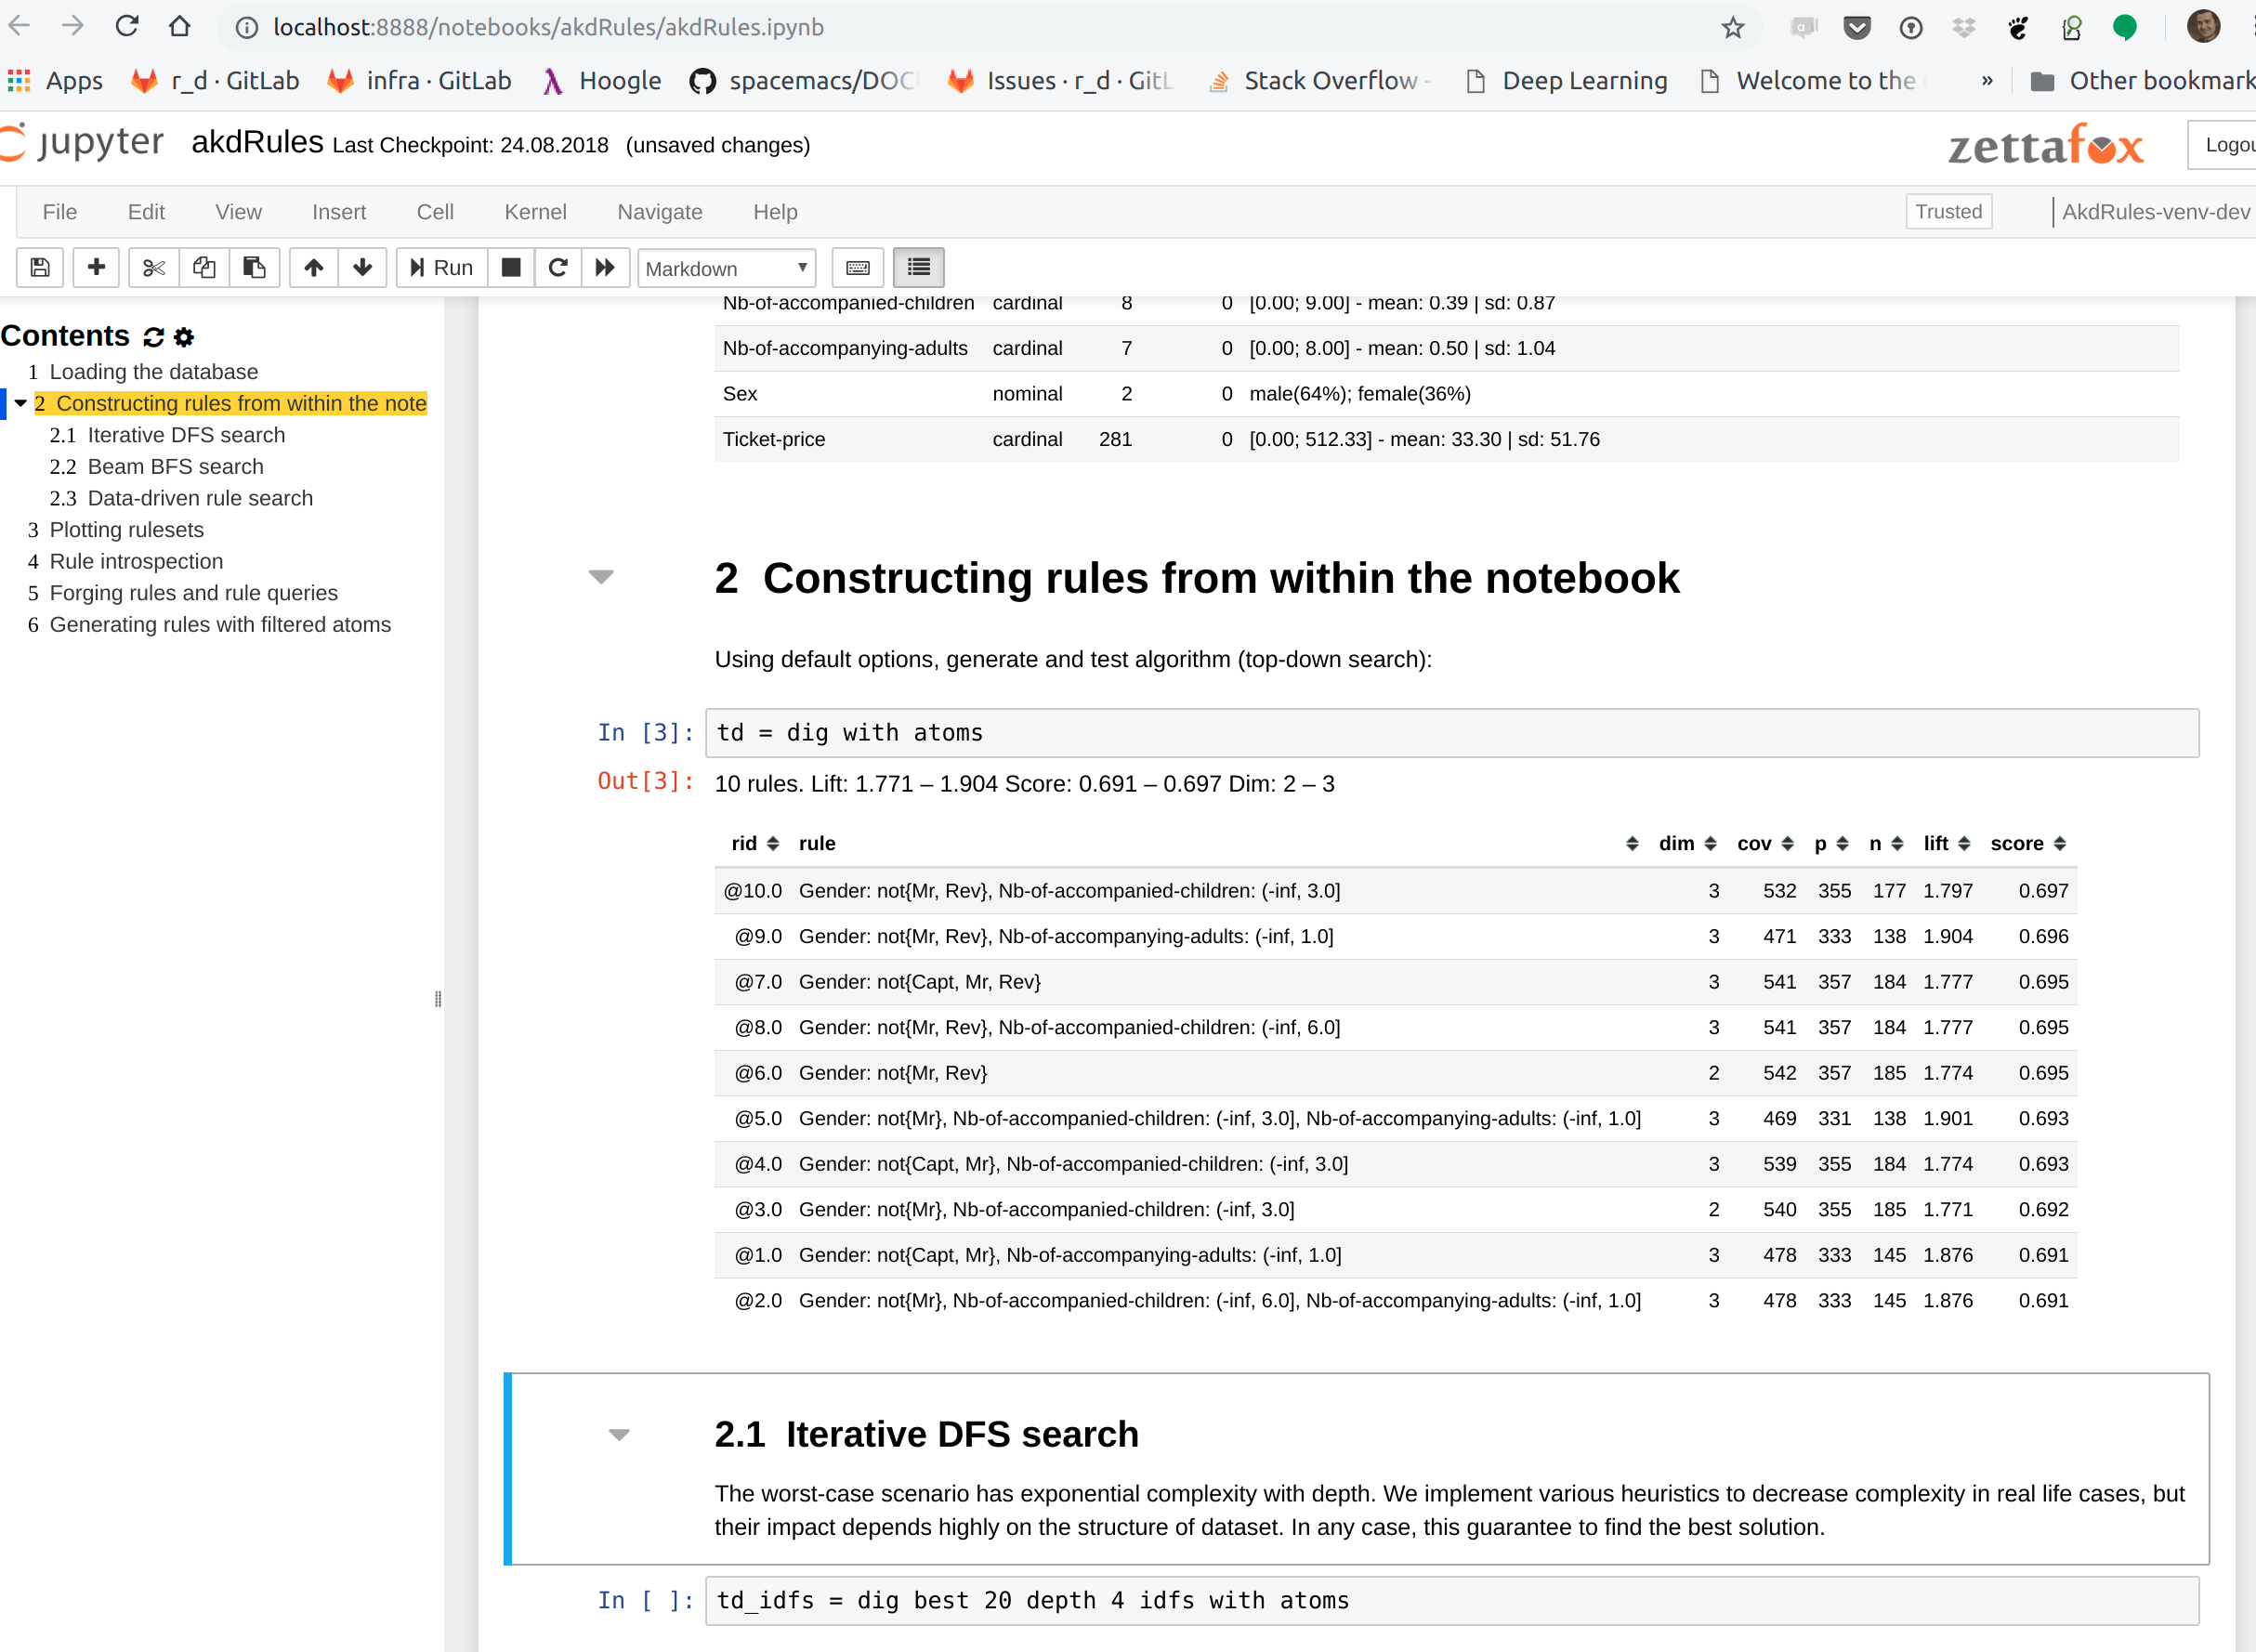
\includegraphics[width=9cm]{jupyter.png}
  \end{center}
  \begin{itemize}
  \item znajomy interfejs
  \item pozwala wykorzystać algorytmy wyszukujące reguły
    do edycji istniejących reguł -- przydatne gdy dodaje
    się wiedzę domenową.
  \end{itemize}
\end{frame}

\section{Podsumowanie}

\begin{frame}
  \frametitle{Podsumowanie}

  Dzięki dopasowaniu specyfiki problemu i cech narzędzia, udało się uzyskać:
  \begin{itemize}
  \item wydajniejszy proces tworzenia narzędzia
  \item kod łatwiejszy w utrzymaniu
  \item łatwość tworzenia eksperymentalnych wariantów
  \item większą szybkość działania
  \item łatwiejsze testowanie
  \item większa satysfakcja z pracy
  \end{itemize}

  Choć bywały trudniejsze momenty:
  \begin{itemize}
  \item brak wsparcia w ekosystemie
  \item nie jest to droga dla początkujących
  \item trzeba uważać na przesadną abstrakcję
  \end{itemize}
\end{frame}

\begin{frame}[standout]
  Dziękuję za uwagę
\end{frame}

\end{document}
